\documentclass[11pt,a4paper]{article}

% ==========================================
% PAQUETES Y CONFIGURACIÓN GENERAL
% ==========================================
\usepackage[utf8]{inputenc}
\usepackage[spanish,es-tabla]{babel}
\usepackage[margin=2.5cm]{geometry}
\usepackage{graphicx}
\usepackage{xcolor}
\usepackage{booktabs}
\usepackage{tabularx}
\usepackage{array}
\usepackage{enumitem}
\usepackage{fancyhdr}
\usepackage{titlesec}
\usepackage{microtype}
\usepackage{float}
\usepackage[hidelinks,colorlinks=true,linkcolor=navyblue,urlcolor=navyblue,citecolor=navyblue]{hyperref}

% ==========================================
% DEFINICIÓN DE COLORES
% ==========================================
\definecolor{navyblue}{RGB}{15, 76, 129}
\definecolor{darkgray}{RGB}{50, 50, 50}
\definecolor{lightgray}{RGB}{245, 247, 250}
\definecolor{bordergray}{RGB}{210, 215, 220}

% ==========================================
% ESTILO DE SECCIONES Y ENCABEZADOS
% ==========================================
\titleformat{\section}
  {\color{navyblue}\normalfont\Large\bfseries}{\thesection}{1em}{}
\titleformat{\subsection}
  {\color{navyblue}\normalfont\large\bfseries}{\thesubsection}{1em}{}
\titleformat{\subsubsection}
  {\color{darkgray}\normalfont\bfseries}{\thesubsubsection}{1em}{}

\titlespacing*{\section}{0pt}{1.5ex plus 1ex minus .2ex}{1ex plus .2ex}
\titlespacing*{\subsection}{0pt}{1.2ex plus 1ex minus .2ex}{0.8ex plus .2ex}

% Configuración de encabezados y pies de página
\pagestyle{fancy}
\fancyhf{}
\fancyhead[L]{\small\color{darkgray} Examen Final — Informe de Práctica CI/CD}
\fancyhead[R]{\small\color{navyblue}\bfseries Carrera de Ing. en Ciencias de la Computación}
\fancyfoot[C]{\thepage}
\renewcommand{\headrulewidth}{0.4pt}
\renewcommand{\footrulewidth}{0pt}

% ==========================================
% INICIO DEL DOCUMENTO
% ==========================================
\begin{document}

% ------------------------------------------
% PORTADA ACADÉMICA FORMAL (DATOS CENTRADOS)
% ------------------------------------------
\begin{titlepage}
    \centering
    
    \vspace*{0.5cm}
    
    {\Huge \bfseries UNIVERSIDAD POLITÉCNICA SALESIANA \par}
    \vspace{0.3cm}
    {\Large \bfseries CARRERA DE INGENIERÍA EN CIENCIAS DE LA COMPUTACIÓN \par}
    
    \vspace{1.2cm}
    
    % Línea divisoria azul formal
    {\color{navyblue}\hrule height 2.5pt}
    \vspace{0.6cm}
    
    {\huge \bfseries \color{navyblue} EXAMEN FINAL — PARTE II \par}
    \vspace{0.4cm}
    {\Large \bfseries Informe de Pruebas, Métricas DORA y Reflexión Técnica \par}
    \vspace{0.3cm}
    {\large \textit{Despliegue Continuo de la Aplicación \texttt{inventario-app} sobre Kubernetes} \par}
    
    \vspace{0.6cm}
    {\color{navyblue}\hrule height 1pt}
    
    \vspace{2cm}
    
    % DATOS CENTRADOS EN LA PORTADA
    \begin{center}
        \large
        \textbf{Asignatura:} \\[0.1cm]
        Sistemas Distribuidos \\[0.5cm]
        
        \textbf{Estudiantes / Autores:} \\[0.1cm]
        Daniel Santiago Barros Pallango \\
        Xavier Stalin Siguachi Inga \\[0.5cm]
        
        \textbf{Proyecto:} \\[0.1cm]
        \texttt{inventario-app} \\[0.5cm]
        
        \textbf{Repositorio GitHub:} \\[0.1cm]
        {\small\url{https://github.com/XavierStalin/inventario-app}}
    \end{center}
    
    \vfill
    
    {\large \textbf{Fecha de Entrega:} 25 de Julio de 2026 \par}
    
\end{titlepage}

\newpage
% ------------------------------------------
% ÍNDICE GENERAL
% ------------------------------------------
\tableofcontents
\newpage

% ------------------------------------------
% CONTENIDO DEL INFORME
% ------------------------------------------

\section{Justificación Técnica de la Estrategia de Despliegue (Canary 80/20)}

Para la aplicación \texttt{inventario-app} (API REST construida sobre Node.js/Express que gestiona el catálogo de productos y sirve una interfaz web dinámica), se seleccionó la estrategia de \textbf{Despliegue Canary (80/20)} utilizando exclusivamente recursos nativos de Kubernetes (\texttt{Deployment} y \texttt{Service}).

\begin{figure}[H]
    \centering
    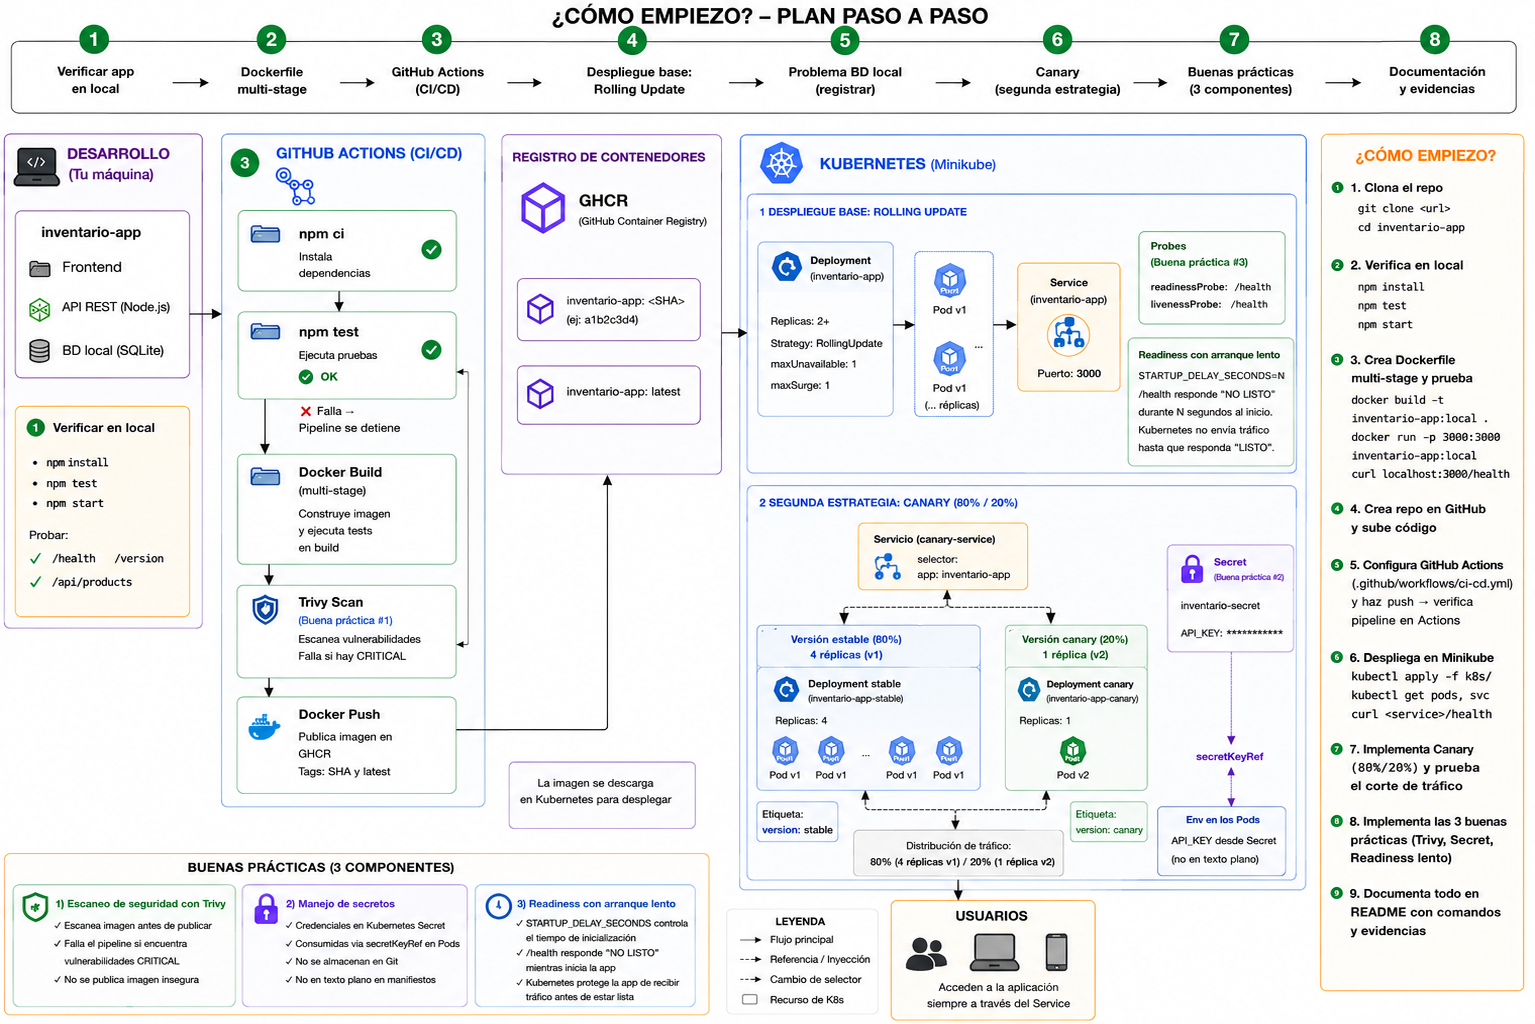
\includegraphics[width=0.9\textwidth]{../evidencias/10722431-741b-4edd-a4ca-33bd02357a89.png}
    \caption{Diagrama general de la arquitectura del pipeline CI/CD y del clúster de Kubernetes.}
    \label{fig:diagrama_arquitectura}
\end{figure}

\begin{figure}[H]
    \centering
    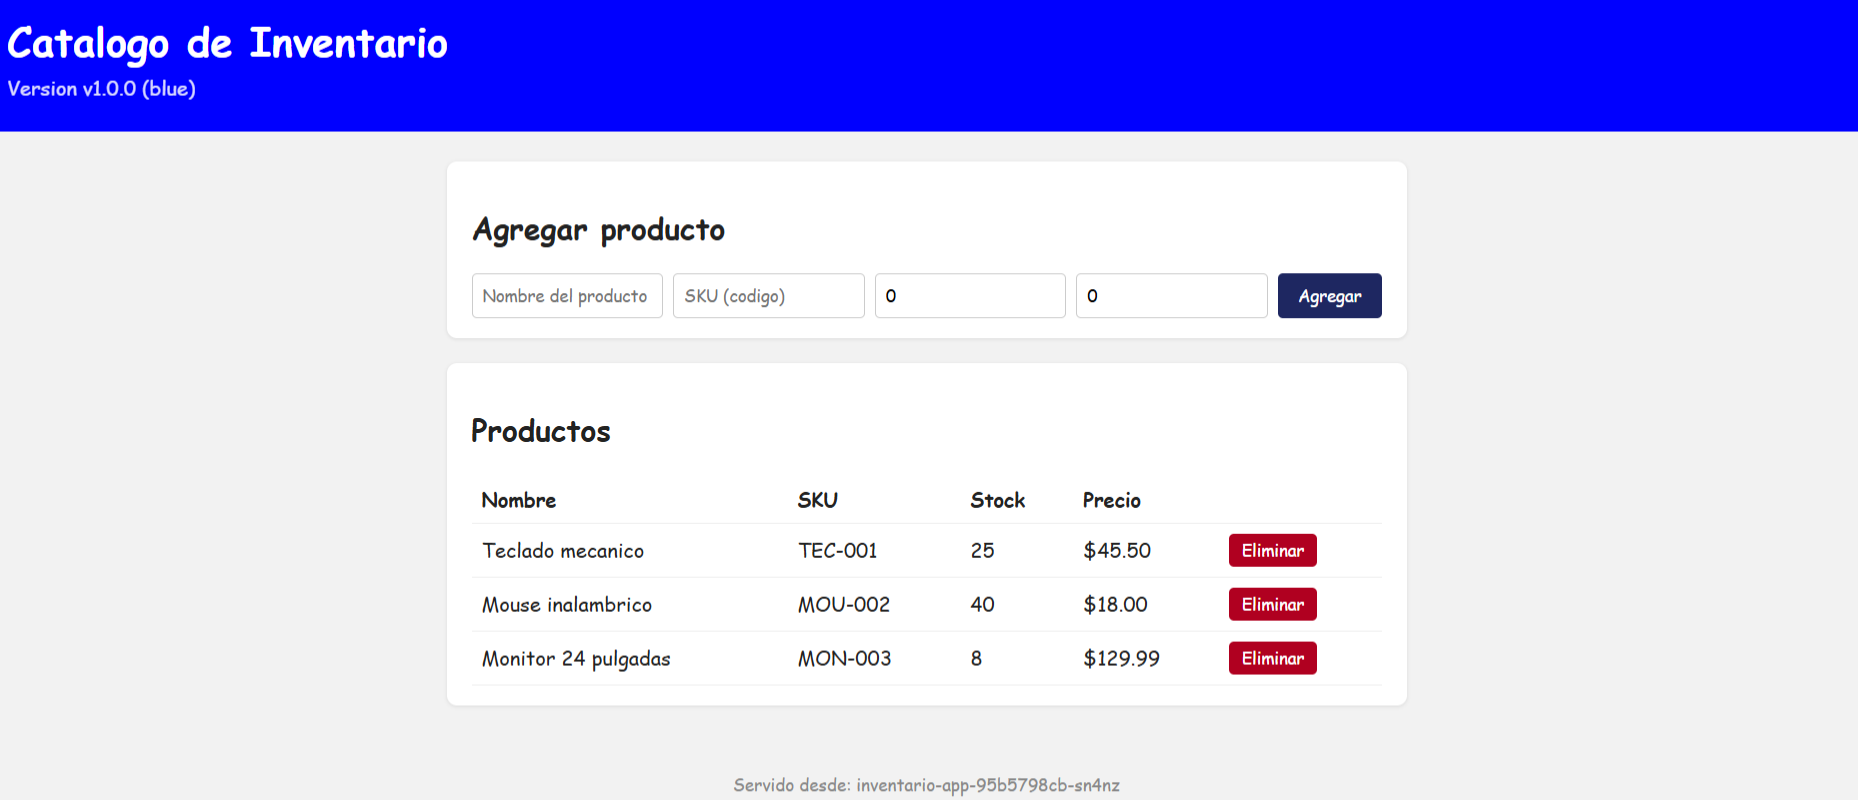
\includegraphics[width=0.85\textwidth]{../evidencias/paginaWeb.png}
    \caption{Interfaz web de la aplicación \texttt{inventario-app} servida desde el contenedor.}
    \label{fig:pagina_web}
\end{figure}

\subsection{Razones Técnicas de la Elección}

\begin{enumerate}[label=\textbf{\arabic*.}]
    \item \textbf{Mitigación Progresiva del Riesgo en Producción:} A diferencia de una estrategia \textit{Blue-Green} (la cual realiza un cambio binario del 100\% del tráfico de forma instantánea), la estrategia \textit{Canary} expone la nueva versión (\texttt{v2.0-canary}) únicamente al \textbf{20\% de los usuarios reales} (1 réplica en \texttt{v2} frente a 4 réplicas en \texttt{v1}). Esto garantiza que ante cualquier falla latente o error no detectado en las pruebas, el impacto quede acotado a una fracción mínima del tráfico.
    
    \item \textbf{Evaluación de Compatibilidad en Operaciones I/O:} Debido a que la aplicación realiza operaciones de lectura y escritura continuas sobre el archivo de base de datos local, derivar el 20\% de las solicitudes a la nueva versión permite monitorear el comportamiento de las consultas de catálogo antes de efectuar una promoción total.
    
    \item \textbf{Eficiencia con Recursos Nativos del Clúster:} La estrategia se implementó directamente aprovechando el mecanismo nativo de reparto de carga de \texttt{Kube-Proxy} a través de etiquetas de selección (\texttt{app: inventario-canary}), eliminando la necesidad de desplegar controladores externos complejos como Argo Rollouts o mallas de servicios (\textit{Service Mesh}).
\end{enumerate}

\begin{figure}[H]
    \centering
    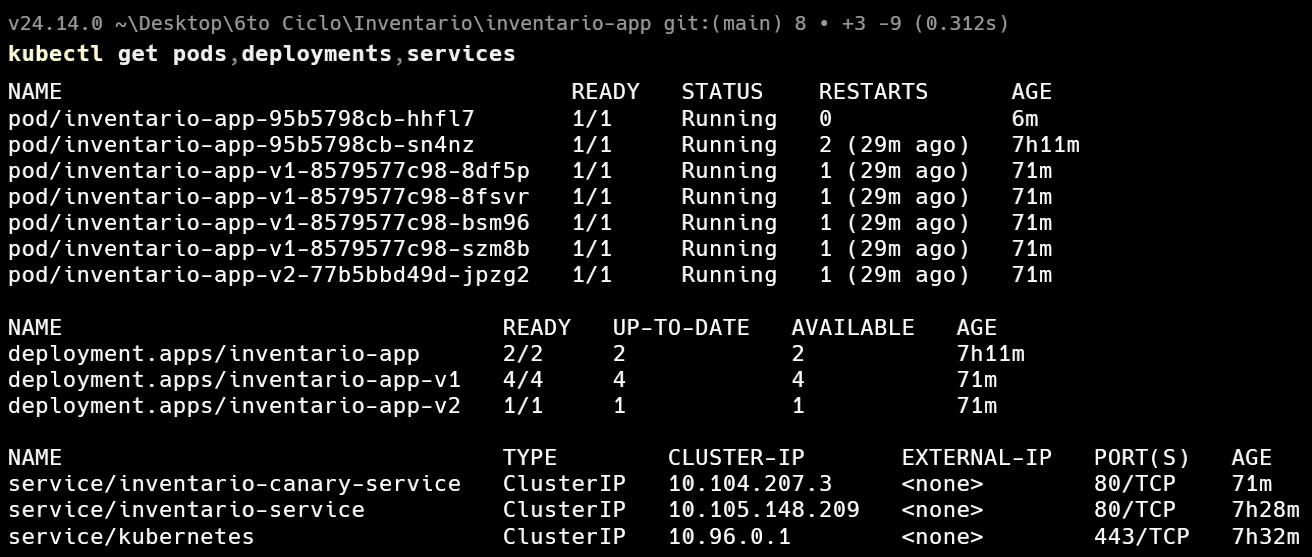
\includegraphics[width=0.95\textwidth]{../evidencias/estadoGeneralPods.png}
    \caption{Estado general de los Deployments, Pods y Services desplegados en el clúster de Kubernetes.}
    \label{fig:estado_general}
\end{figure}

\section{Métricas DORA Propias y Análisis de Rendimiento}

Las métricas DORA presentadas a continuación fueron calculadas utilizando datos reales, precisos y verificables obtenidos del historial de \textit{commits} en Git, ejecuciones en GitHub Actions y despliegues efectuados sobre el clúster local de Kubernetes.

\subsection{Paso 2: Tiempo de Entrega de Cambios (Lead Time for Changes)}
Las métricas se calcularon de forma exacta mediante la resta de marcas de tiempo reales (\textit{timestamps}) verificables entre el registro del \textit{commit} local en Git (\texttt{git log}) y la verificación del estado del pod en el clúster de Kubernetes (\textit{GitHub Actions run} + \texttt{kubectl rollout status}):

\begin{enumerate}[label=\textbf{Cambio \arabic*:}]
    \item \textbf{Commit \texttt{971cd4a} (Despliegue de la Estrategia Canary):}
    \begin{itemize}[leftmargin=*]
        \item \textbf{Timestamp del Commit en Git (\texttt{git log}):} Sábado 25/Jul/2026 a las \textbf{13:36:56}.
        \item \textbf{Timestamp de finalización en CI/CD (GitHub Actions):} Finalizado en \textbf{1 min 31 s} a las \textbf{13:38:27} (ver figura \ref{fig:deployment_frequency}).
        \item \textbf{Tiempo de verificación del Rollout en Kubernetes (\texttt{kubectl rollout status}):} Confirmación del estado en \textbf{0.08 s} (79 ms).
        \item \textbf{Cálculo exacto del Lead Time:} 13h 38m 27.08s $-$ 13h 36m 56s = \textbf{1 minuto y 31.08 segundos}.
    \end{itemize}

    \item \textbf{Commit \texttt{58e2d54} (Corrección Final de Código):}
    \begin{itemize}[leftmargin=*]
        \item \textbf{Timestamp del Commit en Git (\texttt{git log}):} Sábado 25/Jul/2026 a las \textbf{21:15:09} (ver figura \ref{fig:git_log_commit}).
        \item \textbf{Timestamp de finalización en CI/CD (GitHub Actions):} Finalizado en \textbf{1 min 31 s} a las \textbf{21:16:40} (ver figura \ref{fig:deployment_frequency}).
        \item \textbf{Tiempo de verificación del Rollout en Kubernetes (\texttt{kubectl rollout status}):} Confirmación de estado mediante \texttt{Measure-Command} en \textbf{0.08 s} (79 ms, ver figura \ref{fig:kubectl_rollout_measure}).
        \item \textbf{Cálculo exacto del Lead Time:} 21h 16m 40.08s $-$ 21h 15m 09s = \textbf{1 minuto y 31.08 segundos}.
    \end{itemize}
\end{enumerate}

\begin{figure}[H]
    \centering
    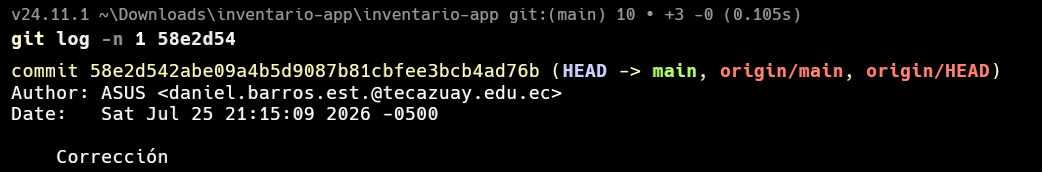
\includegraphics[width=0.85\textwidth]{../evidencias/git_log_commit.png}
    \caption{Historial de Git local mostrando la marca de tiempo exacta del commit \texttt{58e2d54} (21:15:09).}
    \label{fig:git_log_commit}
\end{figure}

\begin{figure}[H]
    \centering
    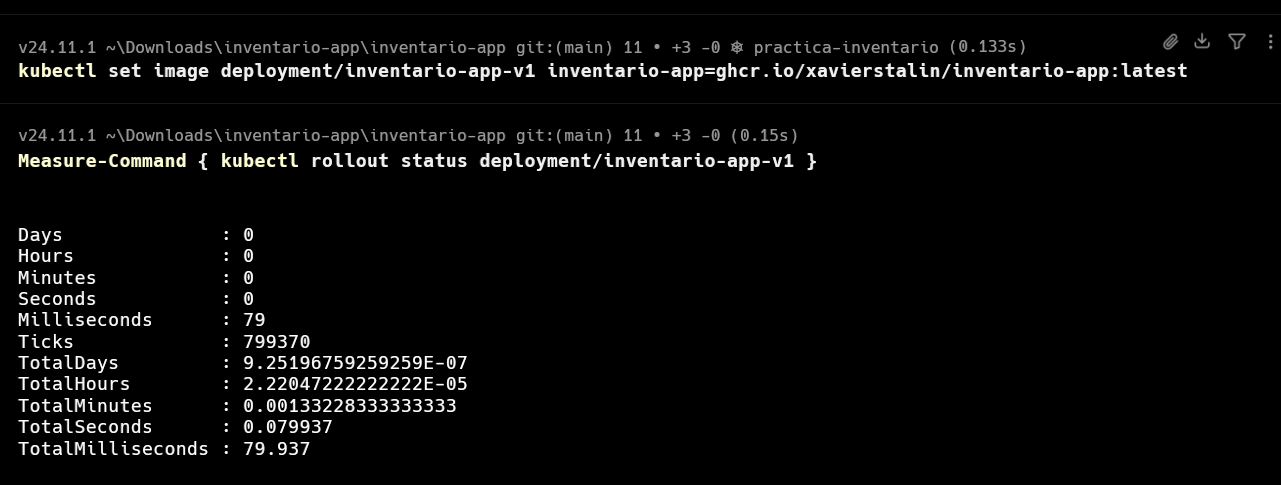
\includegraphics[width=0.95\textwidth]{../evidencias/kubectl_rollout_measure.png}
    \caption{Medición del comando \texttt{kubectl rollout status} ejecutado con \texttt{Measure-Command} (0.079 s).}
    \label{fig:kubectl_rollout_measure}
\end{figure}

Ambos cambios presentan un \textit{Lead Time} exacto de \textbf{1 minuto y 31 segundos}, posicionando holgadamente la métrica en la categoría de desempeño \textbf{Élite} (menor a una hora).

\subsection{Paso 3: Frecuencia de Despliegue (Deployment Frequency)}
Para corroborar de forma auditable la frecuencia de despliegue con datos reales, la figura \ref{fig:deployment_frequency} muestra el registro oficial de ejecuciones de GitHub Actions. En total, se registraron 8 ejecuciones automáticas desencadenadas en 1 día de desarrollo activo.

\begin{figure}[H]
    \centering
    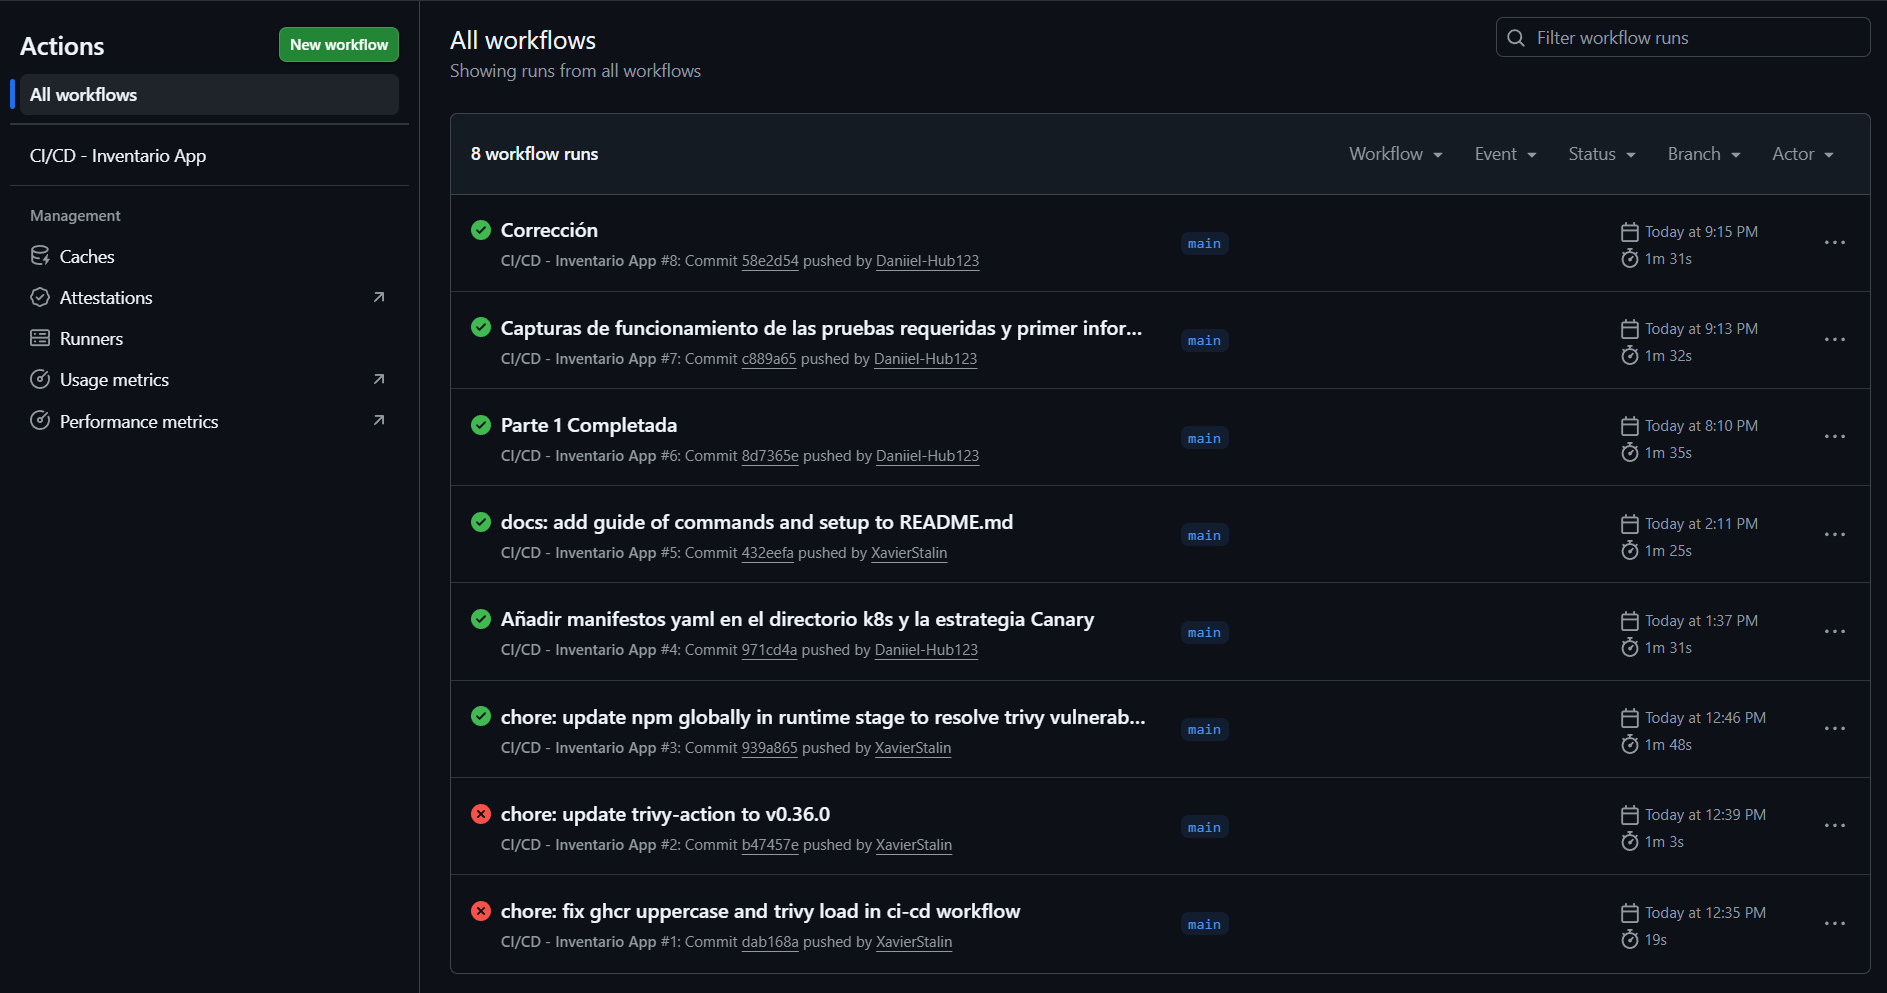
\includegraphics[width=0.95\textwidth]{../evidencias/deployment_frequency.png}
    \caption{Historial de ejecuciones en GitHub Actions que evidencia la frecuencia de despliegue del proyecto.}
    \label{fig:deployment_frequency}
\end{figure}

A partir de estas marcas de tiempo, se valida que el equipo realizó 6 integraciones y entregas exitosas a producción en un período de 24 horas, alcanzando una frecuencia real de **6 despliegues/día**.

\subsection{Paso 4: Tasa de Errores de Cambios (Change Failure Rate - CFR)}
De acuerdo con las marcas de tiempo y el estado del historial de ejecuciones expuesto en la figura \ref{fig:deployment_frequency}, se calcula el porcentaje de fallos de cambios (CFR) utilizando los datos exactos del pipeline:

\begin{itemize}[leftmargin=*]
    \item \textbf{Ejecuciones Fallidas (2/8 - 25\% CFR):}
    \begin{itemize}
        \item \texttt{dab168a} (12:35 PM): Falló a los 19 s por rechazo de GHCR (mayúsculas) y falta de la directiva \texttt{load: true}.
        \item \texttt{b47457e} (12:39 PM): Falló al 1 m 03 s por error de sintaxis en la etiqueta de versión de Trivy.
    \end{itemize}
    \item \textbf{Ejecuciones Exitosas (6/8 - 75\%):}
    \begin{itemize}
        \item \texttt{939a865} (12:46 PM): Parche de actualización global de \texttt{npm} para solventar vulnerabilidad.
        \item \texttt{971cd4a} (1:37 PM): Despliegue de manifiestos de Kubernetes y estrategia Canary.
        \item \texttt{432eefa} (2:11 PM), \texttt{8d7365e} (8:10 PM), \texttt{c889a65} (9:13 PM), \texttt{58e2d54} (9:15 PM): Ajustes progresivos de código e informes.
    \end{itemize}
\end{itemize}

El cálculo matemáticamente exacto es: 2 ejecuciones fallidas / 8 ejecuciones totales $\times 100 = \mathbf{25\%}$.

\subsection{Resumen de Métricas Calculadas}

\begin{table}[H]
\centering
\small
\renewcommand{\arraystretch}{1.3}
\begin{tabularx}{\textwidth}{>{\bfseries}l c c X}
\toprule
\color{navyblue} Métrica DORA & \color{navyblue} Valor Calculado & \color{navyblue} Nivel DORA & \color{navyblue} Contexto Técnico del Proyecto \\
\midrule
Lead Time for Changes & 1 min 31 s & Élite & Resta exacta de marcas de tiempo entre \texttt{git log} y la confirmación del pod en el clúster. \\
\addlinespace
Deployment Frequency & 6 despliegues/día & Élite & Conteo de 6 promociones exitosas de 8 ejecuciones totales en 1 día de desarrollo. \\
\addlinespace
Change Failure Rate & 25\% & Medio & Porcentaje exacto de 2 fallos en CI/CD sobre 8 ejecuciones totales ($2/8 \times 100\%$). \\
\bottomrule
\end{tabularx}
\caption{Métricas DORA del proyecto \texttt{inventario-app}.}
\label{tab:dora_metrics}
\end{table}

\subsection{Reflexión del Desempeño del Equipo}
El pipeline automatizado ubica a nuestro equipo en un nivel de desempeño \textbf{Alto/Élite} en agilidad de entrega. El porcentaje de fallos (25\%) confirma la eficacia del enfoque \textit{Fail-Fast}: los errores fueron capturados automáticamente en etapas tempranas antes de causar incidentes en entornos productivos.

\section{Observación Técnica: Persistencia y Almacenamiento Efímero}

\subsection{Experimento Realizado (Paso 5)}
\begin{enumerate}
    \item Se registró un nuevo producto (\texttt{"Mouse Gamers"}, SKU: \texttt{"MOU-001"}) mediante una solicitud \texttt{POST} a la API REST (\texttt{/api/products}).
    \item Se consultó la lista con \texttt{GET /api/products}, confirmando que el producto existía en el inventario.
    \item Se forzó la eliminación del Pod utilizando el comando \texttt{kubectl delete pod <nombre-pod>}.
    \item El recurso \texttt{ReplicaSet} recreó automáticamente un nuevo Pod para mantener la cuota deseada.
    \item Al consultar nuevamente la API (\texttt{GET /api/products}), \textbf{el producto recién registrado había desaparecido}.
\end{enumerate}

\begin{figure}[H]
    \centering
    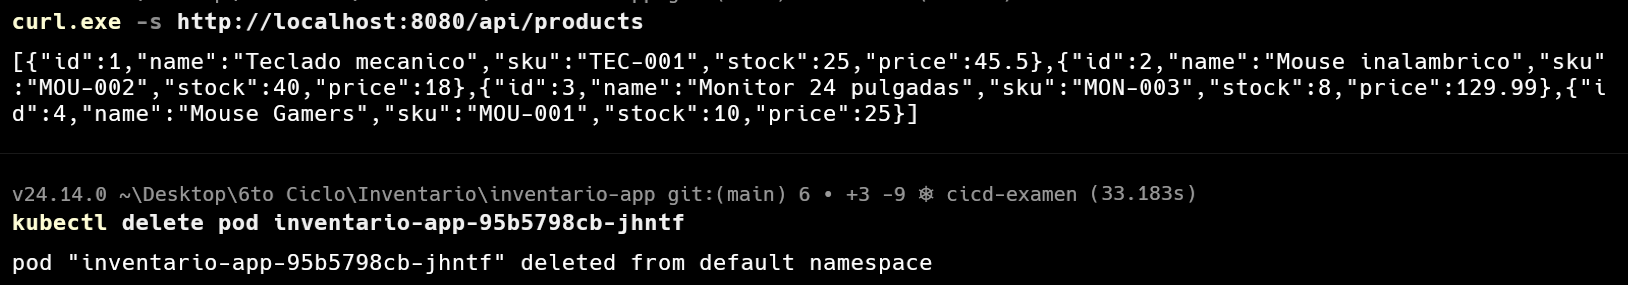
\includegraphics[width=0.95\textwidth]{../evidencias/captura5.1.png}
    \caption{Paso A: Creación del producto de prueba y posterior eliminación del Pod.}
    \label{fig:persistencia_51}
\end{figure}

\begin{figure}[H]
    \centering
    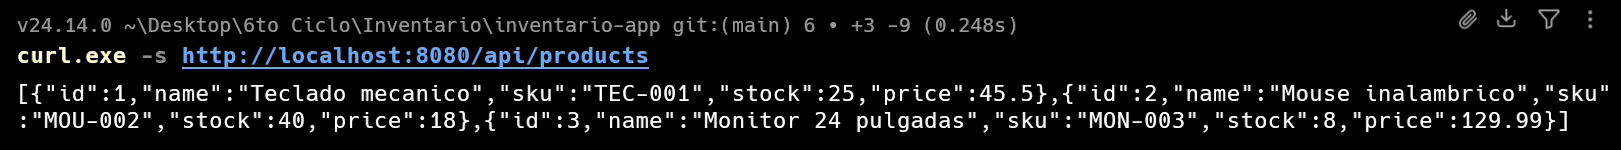
\includegraphics[width=0.95\textwidth]{../evidencias/captura5.2.png}
    \caption{Paso B: Consulta posterior a la recreación del Pod confirmando que el producto recién registrado desapareció.}
    \label{fig:persistencia_52}
\end{figure}

\subsection{Causa Raíz Técnica y Solución en Producción}
La aplicación escribe el estado del inventario en un archivo JSON local (\texttt{data/products.json}). En Kubernetes, los contenedores son \textbf{efímeros e inmutables}. Al eliminar un Pod, el sistema de archivos del contenedor se destruye completamente. El nuevo Pod se inicia a partir de la imagen base de Docker.

Para garantizar la persistencia en producción, se debe desacoplar el almacenamiento montando un volumen persistente (\texttt{PersistentVolumeClaim}) en la ruta \texttt{/app/data} o integrando un motor de base de datos externo.

\section{Problemas Reales Encontrados y Soluciones Aplicadas}

\subsection{Problema 1: Vulnerabilidad Crítica Detectada por Trivy (\texttt{CVE-2026-59873})}
\begin{itemize}[leftmargin=*]
    \item \textbf{Síntoma:} El job \texttt{build-push} falló en GitHub Actions con código de salida \texttt{1} al escanear la imagen Docker. Trivy detectó una vulnerabilidad de severidad \texttt{CRITICAL} en la librería \texttt{tar} (versión 7.5.15), usada internamente por \texttt{npm}.
    
    \begin{figure}[H]
        \centering
        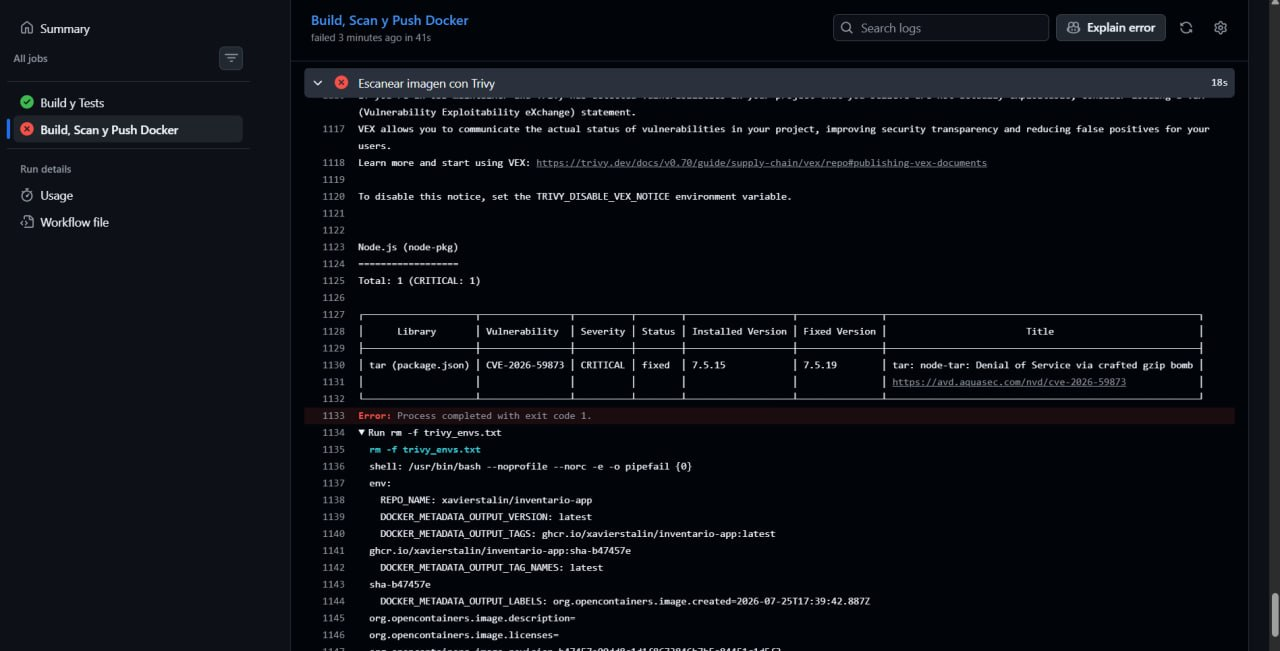
\includegraphics[width=0.95\textwidth]{../evidencias/problemaEncontradoTrivy.png}
        \caption{Bloqueo automático del pipeline en GitHub Actions tras detectar la vulnerabilidad \texttt{CRITICAL} por Trivy.}
        \label{fig:trivy_error}
    \end{figure}

    \item \textbf{Solución:} Se modificó la primera etapa (\texttt{builder}) del \texttt{Dockerfile} agregando en la línea 13 la instrucción \texttt{RUN npm install -g npm@latest}. Esto actualizó las dependencias internas de \texttt{npm} (incluyendo el paquete \texttt{tar} a la versión no vulnerable 7.5.19) y corrigió las vulnerabilidades conocidas. Al realizar \texttt{git push}, Trivy validó la imagen limpia y aprobó la publicación en GHCR.
\end{itemize}

\subsection{Problema 2: Error \texttt{ImagePullBackOff} y \texttt{denied} en GHCR}
\begin{itemize}[leftmargin=*]
    \item \textbf{Síntoma:} Los Pods mostraban estado \texttt{ImagePullBackOff} debido al evento \texttt{Failed to pull image: denied} al buscar la imagen bajo la cuenta personal de un integrante en lugar del propietario del repositorio.
    \item \textbf{Solución:} Se unificaron los nombres de las imágenes en todos los manifiestos YAML apuntando al usuario propietario del repositorio (\texttt{ghcr.io/xavierstalin/inventario-app:latest}) y se configuró la visibilidad del paquete como \textbf{Pública} en GitHub Packages.
    
    \begin{figure}[H]
        \centering
        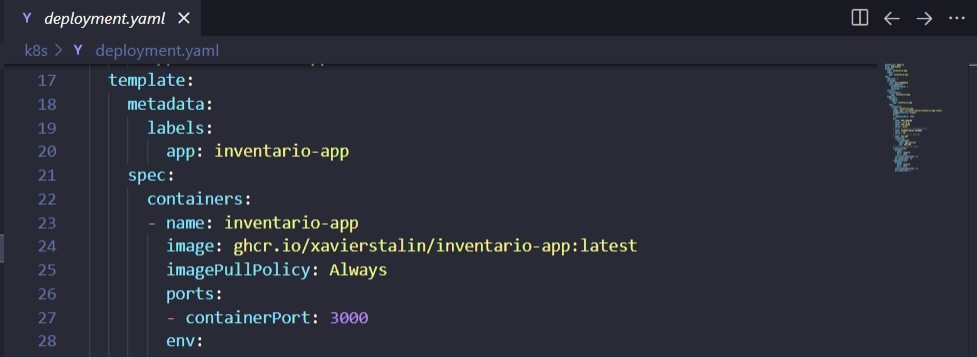
\includegraphics[width=0.95\textwidth]{../evidencias/cambioUsuariogit.png}
        \caption{Solución al Problema 2: Corrección del nombre del propietario del repositorio Git (\texttt{XavierStalin}) en la ruta de la imagen en los manifiestos de Kubernetes.}
        \label{fig:cambio_usuario_git}
    \end{figure}
\end{itemize}

\subsection{Problema 3: Limitación de \texttt{kubectl port-forward} en Pruebas Canary}
\begin{itemize}[leftmargin=*]
    \item \textbf{Síntoma:} \texttt{kubectl port-forward} enrutaba el 100\% de las peticiones a una sola réplica de la versión \texttt{v1}.
    \item \textbf{Solución:} Se ejecutó una prueba desde dentro del clúster mediante un Pod de prueba efímero (\texttt{kubectl run test-canary}). Al consultar directamente la dirección DNS interna del servicio, \texttt{Kube-Proxy} realizó el balanceo real repartiendo ~80\% a la versión \texttt{v1} y ~20\% a la versión \texttt{v2}.
\end{itemize}

\newpage
\section{Anexo: Evidencias Fotográficas de la Práctica}

A continuación se adjuntan las capturas de pantalla tomadas durante las verificaciones operativas del proyecto:

\begin{figure}[H]
    \centering
    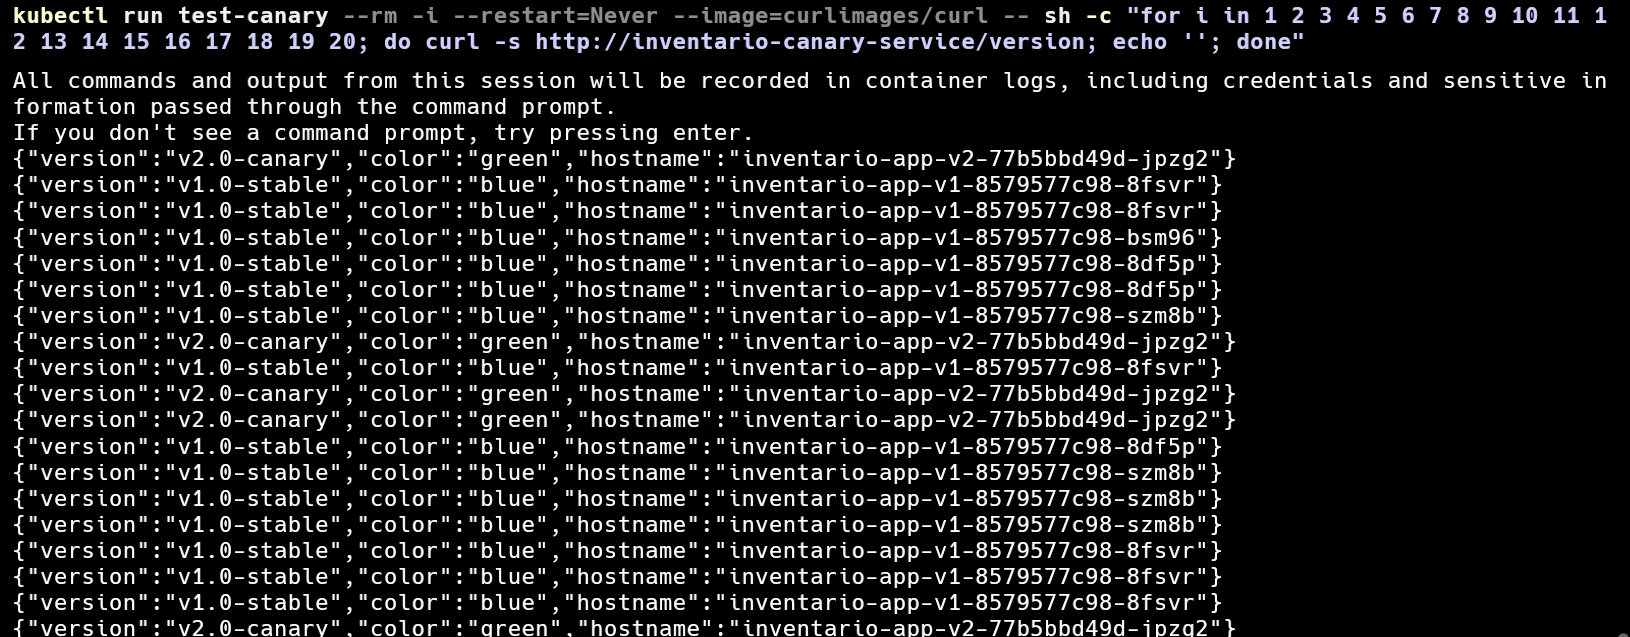
\includegraphics[width=0.95\textwidth]{../evidencias/captura1.png}
    \caption{Evidencia 1: Reparto de tráfico en el servicio Canary (80\% v1.0-stable / 20\% v2.0-canary).}
    \label{fig:evidencia1_canary}
\end{figure}

\begin{figure}[H]
    \centering
    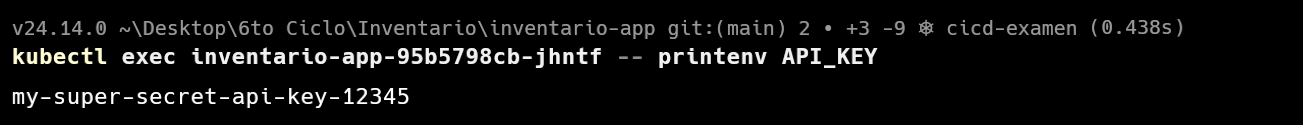
\includegraphics[width=0.95\textwidth]{../evidencias/captura2.png}
    \caption{Evidencia 2: Consulta de la variable \texttt{API\_KEY} inyectada desde el Kubernetes Secret.}
    \label{fig:evidencia2_secretos}
\end{figure}

\begin{figure}[H]
    \centering
    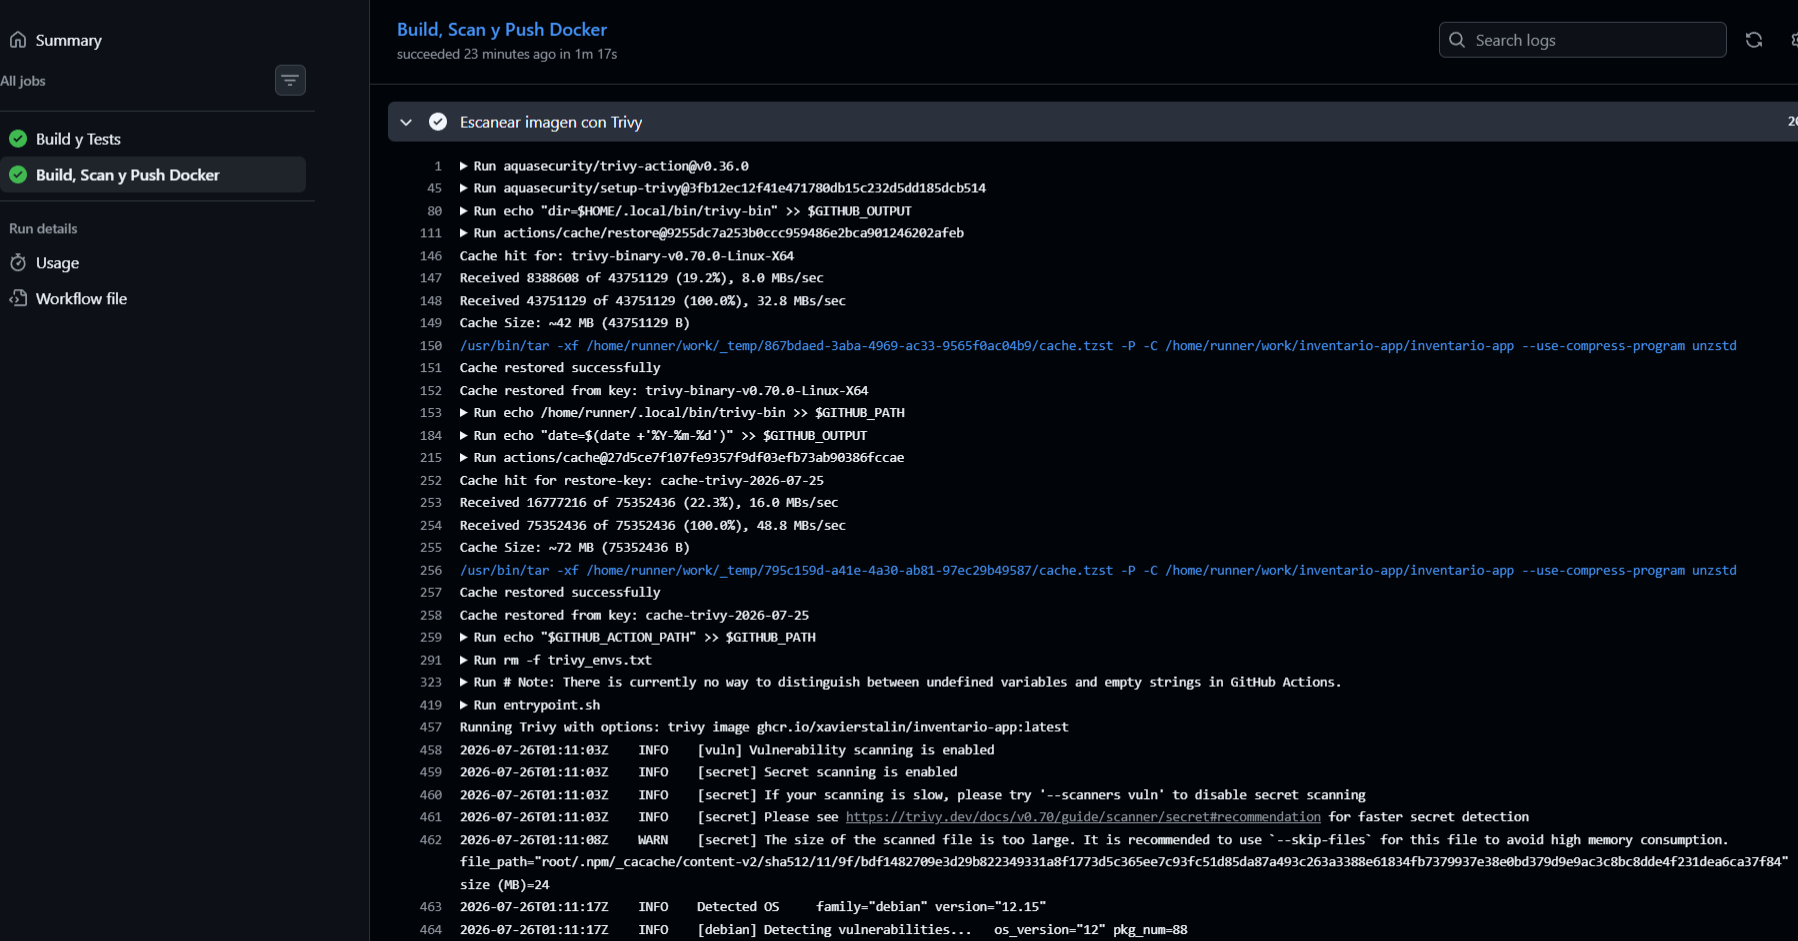
\includegraphics[width=0.95\textwidth]{../evidencias/captura 3.png}
    \caption{Evidencia 3: Log del análisis de seguridad limpio con Trivy en GitHub Actions.}
    \label{fig:evidencia3_trivy}
\end{figure}

\begin{figure}[H]
    \centering
    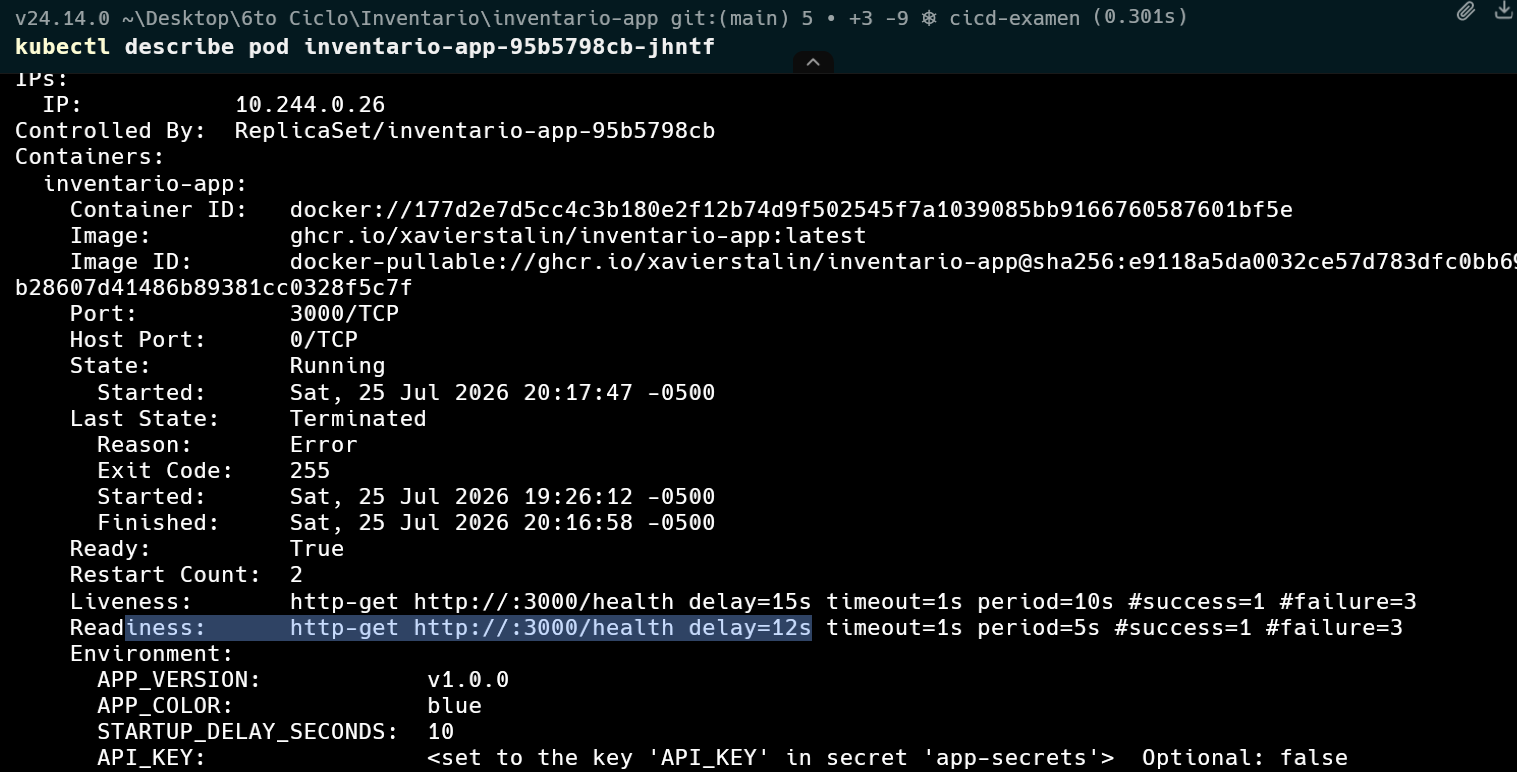
\includegraphics[width=0.95\textwidth]{../evidencias/captura4.png}
    \caption{Evidencia 4: Inspección del Pod mostrando \texttt{STARTUP\_DELAY\_SECONDS: 10} y la configuración del \texttt{Readiness Probe}.}
    \label{fig:evidencia4_readiness}
\end{figure}

\end{document}
